% HERMES: email, files, messages and voice over HF radio (November 2026)
% A 10-minute talk: eleven slides between the title and the thanks.
% Build: make  (pdflatex twice; needs texlive with beamer, metropolis, FiraSans, pgfplots)
% The theme and palette follow Mercury's deck (vendor/mercury/docs/presentations).
% Copyright (C) 2026 Rhizomatica
% SPDX-License-Identifier: CC-BY-SA-4.0
\documentclass[aspectratio=169,10pt]{beamer}

\usetheme[progressbar=frametitle,numbering=fraction,sectionpage=none,block=fill]{metropolis}
\usepackage[sfdefault,lining]{FiraSans}
\usepackage[T1]{fontenc}
\usepackage[utf8]{inputenc}
\usepackage{booktabs,array,colortbl,multirow}
\usepackage{tikz,pgfplots}
\usetikzlibrary{arrows.meta,positioning,calc,shapes.geometric,fit,backgrounds}
\pgfplotsset{compat=1.18}
\usepackage{fontawesome5}

% ---- the HERMES palette (hermes.radio) ------------------------------------
\definecolor{hcream}{HTML}{FFF6C0}
\definecolor{hcreamdk}{HTML}{F6E9A4}
\definecolor{hgreen}{HTML}{96B863}
\definecolor{hdkgreen}{HTML}{5E743E}
\definecolor{horange}{HTML}{FF6600}
\definecolor{hblack}{HTML}{1E1D1D}
\definecolor{hmauve}{HTML}{CD97BD}
\definecolor{hdkmauve}{HTML}{A17895}

\setbeamercolor{normal text}{fg=hblack,bg=hcream}
\setbeamercolor{background canvas}{bg=hcream}
\setbeamercolor{frametitle}{fg=white,bg=hdkgreen}
\setbeamercolor{progress bar}{fg=horange,bg=hgreen}
\setbeamercolor{title separator}{fg=horange}
\setbeamercolor{alerted text}{fg=horange}
\setbeamercolor{example text}{fg=hdkgreen}
\setbeamercolor{block title}{fg=white,bg=hdkgreen}
\setbeamercolor{block body}{fg=hblack,bg=hcreamdk}
\setbeamercolor{block title alerted}{fg=white,bg=horange}
\setbeamercolor{block body alerted}{fg=hblack,bg=hcreamdk}
\setbeamercolor{block title example}{fg=white,bg=hdkmauve}
\setbeamercolor{block body example}{fg=hblack,bg=hcreamdk}
\setbeamercolor{itemize item}{fg=hdkgreen}
\setbeamercolor{itemize subitem}{fg=horange}
\setbeamercolor{page number in head/foot}{fg=hdkgreen}
\setbeamerfont{frametitle}{series=\bfseries,size=\large}
\setbeamerfont{section title}{series=\bfseries}
\setbeamertemplate{itemize item}{\color{hdkgreen}\scriptsize$\blacktriangleright$}
\setbeamertemplate{itemize subitem}{\color{horange}\tiny$\bullet$}
\makeatletter
\setlength{\metropolis@titleseparator@linewidth}{1.5pt}
\setlength{\metropolis@progressonsectionpage@linewidth}{2pt}
\makeatother

% Sources sit on the bottom edge, outside the text area, so they take no room.
\newcommand{\src}[1]{\begin{tikzpicture}[remember picture,overlay]
  \node[anchor=south west,inner sep=0,font=\tiny,text=hdkmauve] at ($(current page.south west)+(0.42cm,0.2cm)$) {#1};
\end{tikzpicture}}
\newcommand{\hl}[1]{{\color{horange}\bfseries #1}}

\title{HERMES}
\subtitle{High-Frequency Emergency and Rural Multimedia Exchange System}
\author{Rhizomatica}
\date{November 2026}

\begin{document}

% ---- title ------------------------------------------------------------------
\begin{frame}[plain]
  \begin{tikzpicture}[remember picture,overlay]
    \fill[hcream] (current page.south west) rectangle (current page.north east);
    \node[anchor=north east,inner sep=0] at (current page.north east)
      {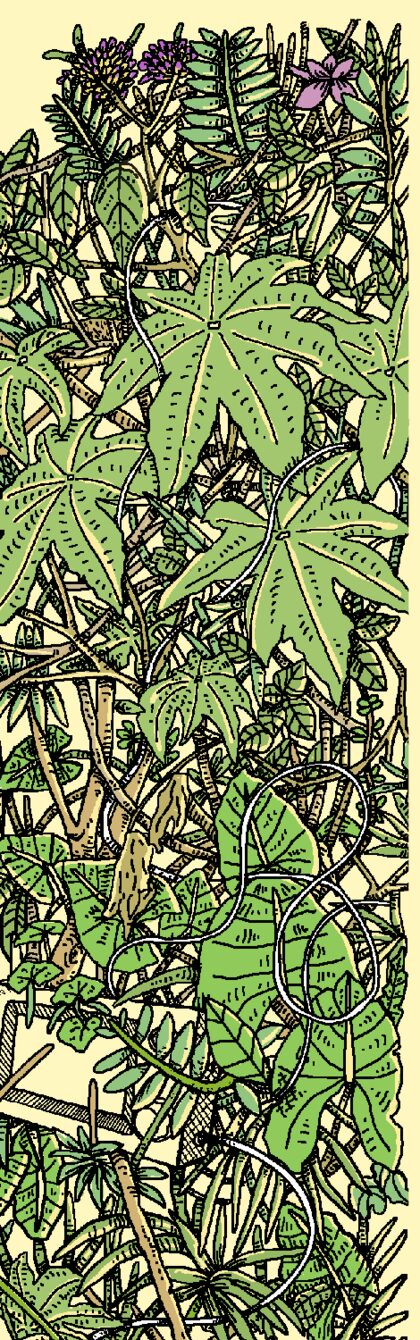
\includegraphics[height=\paperheight]{img/foliage-strip.jpg}};
    \node[anchor=north west,inner sep=0] at ($(current page.north west)+(1.0cm,-0.9cm)$)
      {
\includegraphics[height=2.6cm]{img/hermes-logo.png}};
    \node[anchor=north west,text width=11.2cm,inner sep=0,align=left] at ($(current page.north west)+(1.0cm,-3.8cm)$) {%
      {\fontsize{38}{40}\selectfont\bfseries HERMES}\par\vspace{0.25em}
      {\color{horange}\rule{3.5cm}{2.5pt}}\par\vspace{0.6em}
      {\large High-Frequency Emergency and Rural\\ Multimedia Exchange System}\par\vspace{0.3em}
      {\normalsize Email, files, messages and voice over HF radio,\\ where there is no internet}\par\vspace{0.9em}
      {\small\color{hdkgreen}\bfseries Rhizomatica \quad\textbullet\quad free software \quad\textbullet\quad November 2026}\par
      {\scriptsize\color{hdkmauve}github.com/Rhizomatica \quad\textbullet\quad hermes.radio}};
  \end{tikzpicture}
\end{frame}

\begin{frame}{Overview}
  \small
  \begin{columns}[T]
    \column{0.56\textwidth}
    \begin{itemize}
      \item A \textbf{telecommunication system over HF radio} for communities beyond the reach of the internet and the phone network
      \item People use it as they use the internet: \textbf{email}, webmail and Delta Chat on their phone, over the station's \textbf{WiFi}
      \item The station carries the traffic over \textbf{HF} to a gateway, which has an uplink to the internet
      \item Also \textbf{voice}, digital and encrypted where that is permitted, \textbf{broadcast} files, and \textbf{positions} with an emergency call
      \item \textbf{Free software} from Rhizomatica, supported by ARDC grants since 2021; \textbf{hands-on training} so a community runs its own station
    \end{itemize}
    \column{0.42\textwidth}
    \begin{tikzpicture}[node distance=0.32cm,
        box/.style={draw=hdkgreen,fill=white,rounded corners=2pt,minimum width=4.6cm,minimum height=0.62cm,font=\small,line width=0.8pt},
        acc/.style={box,fill=hgreen!45,font=\small\bfseries}]
      \node[box] (ui) {Phone or laptop \faMobile*\ \faLaptop};
      \node[box,below=of ui] (wifi) {Station WiFi: web UI, mail, chat};
      \node[acc,below=of wifi] (sf) {UUCP \,/\, NNCP store and forward};
      \node[acc,below=of sf] (mod) {Mercury HF modem};
      \node[box,below=of mod] (rd) {hermes-radio-daemon};
      \node[box,below=of rd,fill=hcreamdk] (rad) {SSB transceiver \faBroadcastTower};
      \foreach \a/\b in {ui/wifi,wifi/sf,sf/mod,mod/rd,rd/rad}
        \draw[-{Latex[length=2mm]},hdkgreen,line width=0.8pt] (\a) -- (\b);
    \end{tikzpicture}
  \end{columns}
\end{frame}

\begin{frame}{Where HERMES runs}
  \small
  \begin{columns}[T]
    \column{0.5\textwidth}
    \begin{block}{\faTree\ Ecuadorian Amazon}
      \begin{itemize}
        \item Waorani Indigenous communities: \hl{nearly 90 radios}, the largest deployment
        \item Some sites are days away on foot or by boat
        \item Older residents keep in touch with family in other villages
      \end{itemize}
    \end{block}
    \begin{exampleblock}{\faUsers\ Run by the community}
      Rhizomatica trains a small group of community members, on site, to install, operate and maintain the station without constant outside support
    \end{exampleblock}
    \column{0.46\textwidth}
    \begin{block}{\faShip\ Bangladesh}
      Fishing communities, with HERMES on their \textbf{fishing boats}, in a conservation project
    \end{block}
    \begin{block}{\faExclamationTriangle\ Central African Republic}
      \textbf{Early warning} systems
    \end{block}
  \end{columns}
  \src{Source: ARDC, ``Rhizomatica's HERMES and Mercury Expand Open Source HF Communications'', 6 November 2026}
\end{frame}

\begin{frame}{How a network fits together}
  \centering
  \begin{tikzpicture}[
      box/.style={draw=hdkgreen,fill=white,rounded corners=2pt,align=center,font=\footnotesize,line width=0.8pt,inner sep=5pt},
      acc/.style={box,fill=hgreen!45},
      lnk/.style={{Latex[length=2.2mm]}-{Latex[length=2.2mm]},line width=1pt},
      lab/.style={font=\footnotesize,fill=hcream,inner sep=1.5pt}]
    \node[box,fill=hcreamdk,text width=2.2cm] (net) at (0,0) {\faGlobe\ \textbf{Internet}\\e-mail};
    \node[acc,text width=5.2cm] (cs) at (6,0) {\textbf{Central server} (hermes.radio)\\Postfix + DKIM, UUCP over TCP};
    \node[acc,text width=6.2cm] (gw) at (6,-1.85) {\textbf{Gateway station}\\Postfix, UUCP, scheduled calls, modem, radio};
    \foreach \x/\n in {1.45/a,6/b,10.55/c}
      \node[box,text width=3.9cm] (r\n) at (\x,-4.2) {\textbf{Remote station}\\Postfix, UUCP, modem, radio,\\WiFi access point};
    \draw[lnk,hdkgreen] (net) -- (cs) node[lab,midway,above] {SMTP};
    \draw[lnk,hdkmauve] (cs) -- (gw) node[lab,midway,right] {OpenVPN};
    \foreach \n in {a,b,c} \draw[lnk,horange] (gw) -- (r\n);
    \node[lab,text=horange] at (6,-3.05) {\textbf{HF radio}: Mercury};
  \end{tikzpicture}
  \par\bigskip
  {\footnotesize The central server queues mail for each gateway. The gateway calls the central server over the VPN every few minutes, and its remote stations over HF on schedules set in its web interface.}
  \src{Source: hermes-installer docs/README.md, docs/deploying-a-network.md}
\end{frame}

\begin{frame}{A station}
  \small
  \begin{columns}[T]
    \column{0.5\textwidth}
    \begin{block}{\faMicrochip\ Hardware}
      \begin{itemize}
        \item A \textbf{Raspberry Pi} (1 to 16 GB) or another Debian computer
        \item An \textbf{SSB transceiver}: the \textbf{sBitx} or zBitx, driven directly, or any radio Hamlib controls (IC-7100, IC-7300, FT-710, TS-480, ...)
        \item An antenna, and a WiFi access point for the users
        \item Optionally a GPS receiver
      \end{itemize}
    \end{block}
    \column{0.5\textwidth}
    \begin{block}{\faCogs\ Software}
      \begin{itemize}
        \item Debian 13 and the HERMES package repository
        \item Postfix and Dovecot, UUCP (or NNCP), Mercury, \textbf{hermes-radio-daemon}
        \item A web interface for messages, users, the radio, the UUCP queue and schedules
        \item One installer for every station, from a \textbf{station file}; a USB installer image for the field
      \end{itemize}
    \end{block}
  \end{columns}
  \src{Source: hermes-installer docs/station-files.md; hermes-radio-daemon README.md}
\end{frame}

\begin{frame}{Data over HF: store and forward, and broadcast}
  \small
  \begin{columns}[T]
    \column{0.55\textwidth}
    \begin{itemize}
      \item \textbf{UUCP} carries mail and files over HF by default; it is robust, resumes interrupted transfers, and every station already knows it
      \item \textbf{NNCP}, encrypted and authenticated, is the alternative; a network uses one or the other on every station
      \item The link is \textbf{Mercury}: an ARQ session that delivers a file intact, or reports that it did not
      \item A station keeps mail while the band is closed and sends it at the next call
    \end{itemize}
    \column{0.42\textwidth}
    \begin{block}{Mercury, the link}
      \footnotesize Free software since May 2026, replacing VARA, a proprietary modem with a paid licence per radio. Seven speed rungs, from MFSK below $-10$ dB SNR to 3.1 kbit/s; a VARA-compatible TNC. It has its own presentation.
    \end{block}
    \begin{block}{Broadcast: one to many}
      \footnotesize Files go out as a \textbf{RaptorQ fountain}: a receiver that hears enough of \emph{any} frames rebuilds the file, wherever it tuned in. No return path: bulletins and updates to a whole region.
    \end{block}
  \end{columns}
  \src{Source: hermes-installer docs/README.md; Mercury docs/presentations/2026-10-mercury; hermes-broadcast WIRE-FORMAT.md}
\end{frame}

\begin{frame}{hermes-radio-daemon}
  \footnotesize
  \begin{columns}[T]
    \column{0.52\textwidth}
    \begin{itemize}
      \item \textbf{One daemon} for the radio: control, DSP, audio, voice, digital modes and the modem
      \item Two backends: \textbf{hfsignals} drives the sBitx and zBitx hardware itself (synthesiser, GPIO, codec); \textbf{hamlib} drives any CAT radio
      \item Mercury runs \textbf{inside} it, keyed and fed audio directly
      \item \textbf{One front door}, one HTTPS port: the web interface, REST under \texttt{/api/v2}, the \texttt{hermes.v1} WebSocket, audio over WebRTC
      \item Spec first: \hl{113 operations} in an OpenAPI contract; Go handlers linked into the daemon; every route needs a login, roles enforced on the server
    \end{itemize}
    \column{0.46\textwidth}
    \begin{tikzpicture}[node distance=0.26cm,
        box/.style={draw=hdkgreen,fill=white,rounded corners=2pt,minimum width=5.0cm,minimum height=0.56cm,font=\scriptsize,line width=0.8pt},
        acc/.style={box,fill=hgreen!45,font=\scriptsize\bfseries}]
      \node[box] (ui) {Web UI \,·\, apps \,·\, scripts};
      \node[acc,below=of ui] (api) {HTTPS: /api/v2 REST, hermes.v1, WebRTC};
      \node[acc,below=of api] (core) {Voice \,·\, digital modes \,·\, Mercury \,·\, broadcast};
      \node[acc,below=of core] (dsp) {DSP: SSB, AM, FM, CW, DRM; noise reduction};
      \node[box,below=of dsp] (be) {hfsignals (sBitx) \,|\, hamlib (CAT radios)};
      \node[box,below=of be,fill=hcreamdk] (rad) {Transceiver \faBroadcastTower};
      \foreach \a/\b in {ui/api,api/core,core/dsp,dsp/be,be/rad}
        \draw[{Latex[length=2mm]}-{Latex[length=2mm]},hdkgreen,line width=0.8pt] (\a) -- (\b);
    \end{tikzpicture}
  \end{columns}
  \src{Source: hermes-radio-daemon README.md; docs/api-design/README.md; api/spec/api-rest.yaml}
\end{frame}

\begin{frame}{Digital voice, and encryption where it is permitted}
  \footnotesize
  \begin{columns}[T]
    \column{0.5\textwidth}
    \begin{block}{\faMicrophone\ Two digital voice codecs}
      \begin{itemize}
        \item \textbf{RADE V2}: neural digital voice (FARGAN vocoder, the RADE V2 modem), entirely in C inside the daemon
        \item \textbf{D-STAR}: AMBE voice, compatible with commercial D-STAR radios
        \item A profile switches between analogue and digital voice
      \end{itemize}
    \end{block}
    \column{0.5\textwidth}
    \begin{block}{\faLock\ Voice encryption (opt-in)}
      \begin{itemize}
        \item For networks where encryption is permitted, \textbf{never on amateur bands}
        \item One 256-bit key shared by the network's stations
        \item D-STAR: the voice bits XORed with a ChaCha20 keystream
        \item RADE V2: keyed rotations of the carriers every 40 ms; a late listener locks in about 1 s
      \end{itemize}
    \end{block}
  \end{columns}
  \smallskip
  \begin{exampleblock}{On air, October 2026}
    \footnotesize Both codecs, encrypted and clear, with the right key, the wrong key and none, and a listener joining mid-over: all passed. Listeners heard \textbf{no difference} between encrypted and clear speech.
  \end{exampleblock}
  \src{Source: hermes-radio-daemon README.md (Digital Voice, Voice encryption), dsp/rade\_voice.h, dsp/dstar\_voice.h}
\end{frame}

\begin{frame}{Digital text modes and reception reports}
  \small
  \begin{columns}[T]
    \column{0.5\textwidth}
    \begin{itemize}
      \item \textbf{FT8}: receive and send, a decoder with several passes and signal subtraction
      \item \textbf{JS8}: all four submodes (Normal, Fast, Turbo, Slow), receive and send; free-text messages across several frames
      \item \textbf{CW} and \textbf{RTTY}: decoded as \textbf{skimmers}, every station in the passband at once
      \item One log of everything decoded and sent, read through the API
    \end{itemize}
    \column{0.5\textwidth}
    \begin{itemize}
      \item Received stations reported to \textbf{PSKReporter}, with the station's own position from its GPS
      \item \textbf{DRM}: digital broadcast reception, and transmission: music sent and decoded between two stations
      \item SSB voice processing: equaliser, compressor, limiter; on receive, adaptive noise reduction and AGC
    \end{itemize}
  \end{columns}
  \src{Source: hermes-radio-daemon README.md; dsp/ft8*, dsp/js8*, dsp/pskreporter*}
\end{frame}

\begin{frame}{Positions over the air}
  \small
  \begin{columns}[T]
    \column{0.5\textwidth}
    \begin{block}{\faMapMarker*\ Position beacons}
      \begin{itemize}
        \item A station sends its position on a schedule: from its GPS, or a fixed position typed in
        \item Every station heard is listed with its last position, and drawn on a \textbf{map}
        \item The beacon format is documented byte by byte
      \end{itemize}
    \end{block}
    \begin{alertblock}{\faExclamationTriangle\ SOS}
      An emergency code set by a user goes out in every beacon, more often, until the emergency is declared over
    \end{alertblock}
    \column{0.5\textwidth}
    \begin{block}{\faRoute\ Tracks}
      \begin{itemize}
        \item The station's own track, and every other station's from its beacons
        \item A point every few seconds while moving; one every 5 minutes while still
        \item Fixed \textbf{24-byte records}, one file per period: a time range is found by binary search
        \item A \textbf{trip} is a named time range of a track
      \end{itemize}
    \end{block}
  \end{columns}
  \src{Source: docs/BEACON-FORMAT.md, gps/gps\_track.h, api/spec/api-rest.yaml (tag gps)}
\end{frame}

\begin{frame}{Testing and platforms}
  \small
  \begin{columns}[T]
    \column{0.5\textwidth}
    \begin{block}{\faVial\ Testing}
      \begin{itemize}
        \item \textbf{280 C unit tests} (Unity + fff): DSP, codecs, modes, beacons, tracks
        \item \textbf{Go}: every API handler, its refusals too
        \item \textbf{Integration}: the real daemon on Hamlib's dummy radio
        \item \textbf{Sanitizers} (ASan + UBSan, TSan) and CI on amd64 and arm64 for every pull request
        \item \textbf{On air}: sBitx, IC-7100 and FT-710 stations
      \end{itemize}
    \end{block}
    \column{0.5\textwidth}
    \begin{block}{\faServer\ Platforms}
      \begin{itemize}
        \item \textbf{Raspberry Pi} 4 and 5, Debian 13, from the HERMES package repository; Mercury even on a Pi Zero, with the zBitx
        \item \textbf{A phone as the station}: the daemon and Mercury on Sailfish OS and a PinePhone Pro, the radio on USB (CAT without kernel drivers, proposed to Hamlib), the phone's own GPS
        \item Mercury also on \textbf{Android} and \textbf{iOS} phones, \textbf{macOS} and \textbf{Windows}; iOS gives apps no USB access
      \end{itemize}
    \end{block}
  \end{columns}
  \src{Source: tests/, .github/workflows; hermes-radio-daemon README.md; Hamlib pull request 2272}
\end{frame}

\begin{frame}{2026, and what comes next}
  \begin{columns}[T]
    \column{0.46\textwidth}
    \begin{tikzpicture}
      \foreach \v/\l/\y in {580/{commits to the radio\\ daemon since 25 April}/0,
                            117/{pull requests merged in it}/-1.15,
                            1468/{commits to Mercury since its C rewrite}/-2.3,
                            12/{stations in a network\\ installed in November}/-3.45}{
        \node[anchor=east,font=\fontsize{26}{26}\selectfont\bfseries,text=horange] at (1.7,\y) {\v};
        \node[anchor=west,text width=3.7cm,align=left,font=\footnotesize] at (1.95,\y) {\l};
      }
    \end{tikzpicture}
    \column{0.52\textwidth}
    \footnotesize
    \begin{block}{\faExchange*\ Store and forward}
      UUCP and NNCP behind one layer of the station API; SOS messages
    \end{block}
    \begin{block}{\faDesktop\ One interface}
      The web interfaces on the station API; the old WebSocket retired
    \end{block}
    \begin{block}{\faBroadcastTower\ Sharing the channel}
      HF channel access between stations; Mercury's optional encryption
    \end{block}
    \begin{block}{\faProjectDiagram\ Other networks}
      Reticulum over HF (done); Meshtastic, for LoRa networks (in progress)
    \end{block}
  \end{columns}
  \src{Source: git history of hermes-radio-daemon and Mercury; ARDC, 6 November 2026}
\end{frame}

\begin{frame}[plain]
  \begin{tikzpicture}[remember picture,overlay]
    \fill[hcream] (current page.south west) rectangle (current page.north east);
    \node[anchor=north east,inner sep=0] at (current page.north east)
      {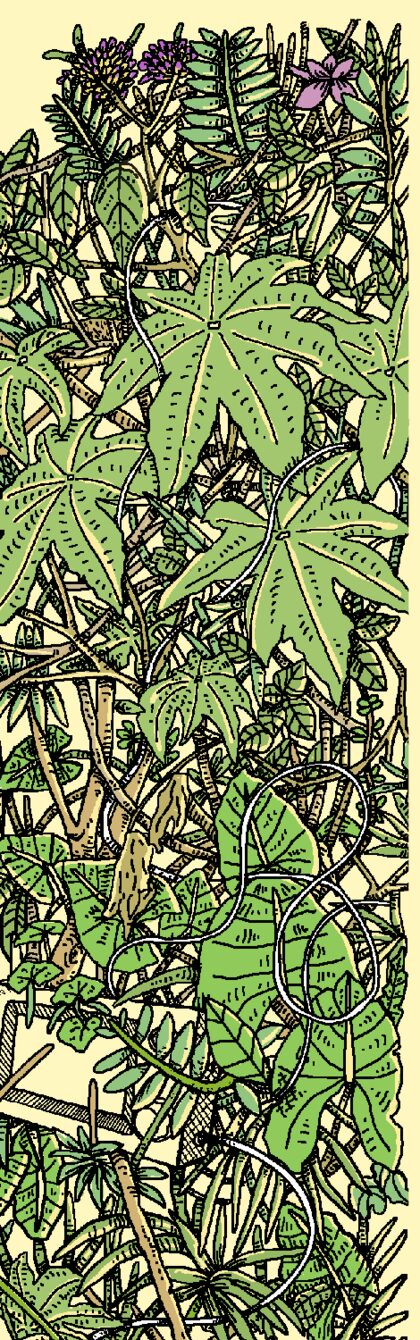
\includegraphics[height=\paperheight]{img/foliage-strip.jpg}};
    \node[anchor=north west,inner sep=0] at ($(current page.north west)+(1.0cm,-1.0cm)$)
      {
\includegraphics[height=2.2cm]{img/hermes-logo.png}};
    \node[anchor=north west,text width=8.6cm,inner sep=0] at ($(current page.north west)+(1.0cm,-4.0cm)$) {%
      {\fontsize{30}{32}\selectfont\bfseries THANK YOU}\par\vspace{0.25em}
      {\color{horange}\rule{3.5cm}{2.5pt}}\par\vspace{0.8em}
      \small
      \faGithub\ \ github.com/Rhizomatica\par\vspace{0.3em}
      \faGlobe\ \ hermes.radio \quad\textbullet\quad rhizomatica.org/hermes\par\vspace{0.3em}
      \faEnvelope\ \ lists.riseup.net/www/info/hermes-general\par\vspace{1.0em}
      {\scriptsize\color{hdkmauve}HERMES is free software.\\ This presentation: CC BY-SA 4.0.}};
  \end{tikzpicture}
\end{frame}

\end{document}
